\documentclass{beamer}
%
% Choose how your presentation looks.
%
% For more themes, color themes and font themes, see:
% http://deic.uab.es/~iblanes/beamer_gallery/index_by_theme.html
%
\mode<presentation>
{
  \usetheme{default}      % or try Darmstadt, Madrid, Warsaw, ...
  \usecolortheme{default} % or try albatross, beaver, crane, ...
  \usefonttheme{default}  % or try serif, structurebold, ...
  \setbeamertemplate{navigation symbols}{}
  \setbeamertemplate{caption}[numbered]
} 

\usepackage[francais]{babel}
\usepackage[utf8]{inputenc}
\usepackage[T1]{fontenc}
\usetheme{Boadilla}
\usepackage{amsmath}

\usepackage[backend=biber,style=authoryear-comp,uniquename=init,firstinits=true,
            %% "et al" pour > deux auteurs, & pour exactement 2
            uniquelist=false,maxcitenames=2,mincitenames=1,maxbibnames=99,
            isbn=false,url=false,doi=false
]{biblatex}


\renewcommand{\cite}{\parencite}
\renewcommand*{\nameyeardelim}{\addcomma \addnbspace}
\renewcommand*{\revsdnamedelim}{}
\renewcommand*\finalnamedelim{ \& }

\DefineBibliographyExtras{french}{\restorecommand\mkbibnamelast}

\DeclareNameAlias{default}{last-first}
\DeclareNameAlias{sortname}{last-first}

% Supprimer les guillemets dans les titres
\DeclareFieldFormat[article,incollection,unpublished,inproceedings]{title}{#1}

% Je n'aime pas, mais j'ai l'impression que mlapafr utilise ça
\renewbibmacro{in:}{\printtext{In} \addspace}


% Espaces insécables dans les citations et la bibliographie (noms de
% conférences) ?

\usepackage{xpatch}
\usepackage{xstring}
%\xpatchbibmacro{series+number}{\addspace}{\addnbspace}{}{}

\renewbibmacro*{series+number}{%
  \setunit*{\addnbspace}%
  \printfield{series}%
  \printfield{number}%
  \newunit}

\newcommand{\beamcite}[1]{\hfill {\footnotesize \textcite{#1}}}


%%%%%%%%%%%%%%%%%%%%%%%%


\addbibresource{references.bib}


\title[Classification monotone]{Apprentissage et classification monotone}
\author{Laura Nguyen}
\institute{LFI}
\date{19 juillet 2018}

\newcommand{\myfrac}[2]{\frac{\displaystyle {#1}}{\displaystyle {#2}}}

\begin{document}

\begin{frame}
  \titlepage
\end{frame}

% Uncomment these lines for an automatically generated outline.
%\begin{frame}{Outline}
%  \tableofcontents
%\end{frame}

\section{Introduction}

\begin{frame}{Classification monotone}
\begin{itemize}
\item Garantie d'une monotonie de la classe par rapport aux valeurs d'attributs
\item Concepts sémantiques : préférence, priorité, importance...
\item Applications : 
    \begin{itemize}
        \item Prédiction du risque de faillite
        \item Evaluation du prix de biens immobiliers
        \item Cote de crédit 
    \end{itemize}
\item Gain en interprétabilité (y compris auprès des experts) et en taux de bonne classification quand le domaine s'y prête\beamcite{pazzani-acceptance}
\end{itemize}
\end{frame}

\begin{frame}{Exemple de problème de classification monotone}
\beamcite{potharst-classification-bank}

\begin{table}
\resizebox{\textwidth}{!}{
\begin{tabular}{|*{5}{c|}}
    \hline
        client & revenu & éducation & casier judiciaire & prêt \\
    \hline 
        cl1 & faible & faible & juste & non\\
        cl2 & faible & faible & excellent & faible\\
        cl3 & moyen & intermédiaire & excellent & intermédiaire\\
        cl4 & élevé & faible & excellent & élevé\\
        cl5 & élevé & intermédiaire & excellent & élevé\\
    \hline
\end{tabular}}
\label{tab:bank-loan-dataset}
\end{table}

\end{frame}

\begin{frame}{Formalisation}

\begin{itemize}
\item Entrées :  
\begin{itemize}
	\item n exemples : $\Omega = \{\omega_1, ... , \omega_n\}$
    \item m attributs ordonnés : $A = (a_1, ... , a_m)$. \\ Pour $j=1,... ,m :$
    	\begin{itemize}
    	\item $a_j : \Omega \rightarrow X_j$ avec $X_j$ totalement ordonné
        \item Espace de description $X = X_1 \times ... \times X_m$
    	\end{itemize}
    \item k classes : $C = {c_1, ... , c_k}$
\end{itemize}
\item Sortie : 
\begin{itemize}
\item Fonction de classification monotone $\lambda : X \rightarrow C$
\end{itemize}
\end{itemize}

\end{frame}

\begin{frame}{Dataset artificiel à un attribut monotone}

\begin{figure}
	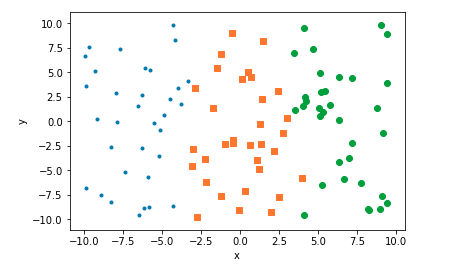
\includegraphics[width=.7\textwidth]{Capture_d__cran_de_2018-07-11_20-06-25.png}
\end{figure}

\end{frame}

\begin{frame}{Classification par arbres de décision}
\begin{itemize}
\item Pas d'hypothèse sur les données
\item Exploiter au mieux l'éventuelle gradualité
\item Classification par arbres de décision 
\begin{itemize}
\item Choisir $a_j$ respectant le plus la contrainte de monotonie locale: \\~\

$\forall \omega_i, \omega_h \in \Omega, a_j(\omega_i) \leq a_j(\omega_h) \Rightarrow \lambda(\omega_i) \leq \lambda(\omega_h)$ \\~\

\item Pas de garantie d'avoir un classifieur globalement monotone

\end{itemize}
\end{itemize}

\end{frame}

\begin{frame}{Mesures de discrimination à rang}
\begin{itemize}
\item Problème : incapacité des mesures de discrimination classiques à détecter la monotonie 
\item Chercher des mesures de discrimination sensibles à la monotonie et robustes au bruit non-monotone
\begin{itemize}
\item Généralisation à rang de mesures classiques (Shannon, Gini)
\item Modèle de construction hiérarchique 
\end{itemize}
\end{itemize}
\end{frame}

\begin{frame}{Ensembles dominants}
\begin{itemize}
\item Classes d'équivalence générés par, : 
\begin{itemize}
\item un attribut $a_j$ : $[\omega_i]_{a_j} = \{\omega_h \in \Omega : a_j(\omega_i) = a_j(\omega_h)\}$
\item la classe $\lambda$ : $[\omega_i]_{\lambda} = \{\omega_h \in \Omega : \lambda(\omega_i) = \lambda(\omega_h)\}$
\end{itemize}

\item Ensembles dominants générés par, :
\begin{itemize}
\item un attribut $a_j : [\omega_i]^{\leq}_{a_j} = \{\omega_h \in \Omega : a_j(\omega_i) \leq a_j(\omega_h)\}$
\item la classe $\lambda$ : $[\omega_i]^{\leq}_{\lambda} = \{\omega_h \in \Omega : \lambda(\omega_i) \leq \lambda(\omega_h)\}$
\end{itemize}

\end{itemize}
\end{frame}

\begin{frame}{Généralisation à rang de l'entropie de Shannon}
\begin{itemize}
\item Entropie conditionnelle de Shannon: 

$H_s(\lambda | a_j) = \sum_{i=1}^{|\Omega|} \frac{1}{|\Omega|}(\log (\frac{|[\omega_i]_{\lambda} \cap [\omega_i]_{a_j}|}{|[\omega_i]_{a_j}|}))$

\item Entropie de Shannon à rang: 

$H^*_s(\lambda | a_j) = \sum_{i=1}^{|\Omega|} \frac{1}{|\Omega|}(\log (\frac{|[\omega_i]^{\leq}_{\lambda} \cap [\omega_i]^{\leq}_{a_j}|}{|[\omega_i]^{\leq}_{a_j}|}))$

\end{itemize}

\end{frame}

\begin{frame}{Modèle de construction hiérarchique de mesures de discrimination à rang \beamcite{marsala-rank}}
\begin{itemize}
\item Isoler les propriétés d'une telle mesure
\item Créer de nouvelles mesures
\item Structure fonctionnelle commune avec 3 fonctions \\
Pour $a_j$ fixé :
\begin{itemize}
\item $f^*$ : mesure de monotonie locale de l'objet
\item $g^*$ : mesure de non-monotonie locale de l'objet
\item $h^*$ : agrégation de mesures de non-monotonie locale
\end{itemize}
Ecriture générique : \\~\
$H^*(\lambda | a_j) = h^*(g^*(f^*(\omega_1)),...,g^*(f^*(\omega_n)))$
\end{itemize}
\end{frame}


\begin{frame}{Couche $f^*$}
    Pour $a_j \in A$ fixé,
    \begin{itemize}
        \item $dsr(\omega_i) = \myfrac{| [\omega_i]^{\leq}_{\lambda} \cap [\omega_i]^{\leq}_{a_j}|}{| [\omega_i]^{\leq}_{a_j} |}$
        \item $mindsr(\omega_i) = \myfrac{min_{\omega_h \in [\omega_i]_{a_j}} |[\omega_h]^{\leq}_{\lambda} \cap [\omega_h]^{\leq}_{a_j}|}{| [\omega_i]^{\leq}_{a_j} |}$
        \item $maxdsr(\omega_i) = \myfrac{max_{\omega_h \in [\omega_i]_{a_j}} |[\omega_h]^{\leq}_{\lambda} \cap [\omega_h]^{\leq}_{a_j}|}{| [\omega_i]^{\leq}_{a_j} |}$
        \item $avgdsr(\omega_i) = \myfrac{\displaystyle\sum_{\omega_h \in [\omega_i]_{a_j}} \myfrac{|[\omega_h]^{\leq}_{\lambda} \cap [\omega_h]^{\leq}_{a_j}|}{|[\omega_i]_{a_j}|}}{| [\omega_i]^{\leq}_{a_j} |}$
    \end{itemize}
\end{frame}

\begin{frame}{Réécriture des mesures de discrimination à rang}
    \begin{itemize}
        \item $H^*_S(\lambda|a_j) = \displaystyle\sum_{i=1}^{n}\myfrac{1}{n} (-\log(dsr(\omega_i)))$
        \begin{itemize}
            \item $f^*_S = dsr(\omega_i)$
            \item $g^*_S = -\log(f^*_S(\omega_i))$
            \item $h^*_S = \sum_{i=1}^{n} \myfrac{1}{n} g^*_S(f^*_S(\omega_i))$
        \end{itemize}
        \item $H^*_P(\lambda|a_j) = \displaystyle\sum_{i=1}^{n}\myfrac{1}{n} (-\myfrac{\log(mindsr(\omega_i))}{mindsr(\omega_i)})$
        \begin{itemize}
            \item $f^*_P = mindsr(\omega_i)$
            \item $g^*_P = -\myfrac{\log f^*_P(\omega_i)}{f^*_P(\omega_i)}$
            \item $h^*_P = \sum_{i=1}^{n} \myfrac{1}{n} g^*_P(f^*_P(\omega_i))$
        \end{itemize}
    \end{itemize}
\end{frame}

\begin{frame}{Construction d'arbres de décision monotones \beamcite{marsala-rank}}
    \begin{itemize}
        \item Classifieur RDMT(H) paramétré par : 
            \begin{itemize}
                \item Une mesure de discrimination H
                \item 3 critères de pré-élagage : partitionnement, arrêt, étiquetage
            \end{itemize}
        \item Critère de partitionnement (splitting rule)
            \begin{itemize}
                \item Chaque attribut $a_j$ est binarisé : $\forall x \in X_j$,
                    \begin{equation*}
                    \begin{array}{cl}
                        a^x_j(\omega_i) = \begin{cases}{0} &\text{ if } a_j(\omega_i) \leq x\\
                          {1} &\text{ otherwise}\end{cases}
                     \end{array}
                     \end{equation*}
                \item Trouver $a^{x_*}_*$ minimisant $H(\lambda|a^x_j)$
                    \begin{itemize}
                        \item $a_*$ est l'attribut utilisé pour le partionnement
                        \item $x_*$ est la valeur seuil : 
                            \begin{equation*}
                            \begin{array}{cl}
                                x_* = arg\,min \{H(\lambda|a^x) | j=1,...,m, x \in X_j\}
                            \end{array}
                            \end{equation*}
                    \end{itemize}
            \end{itemize}
    \end{itemize}
\end{frame}

\begin{frame}{Critère de partitionnement}
    \begin{figure}
	    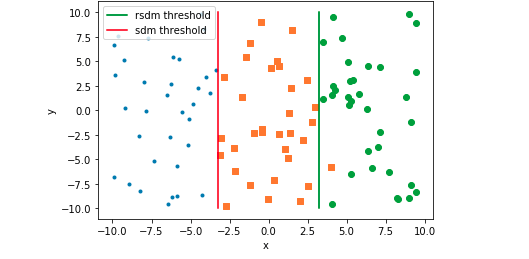
\includegraphics[width=.7\textwidth]{split.png}
    \end{figure}
\end{frame}

\begin{frame}{Arbres de décision générés}
    \begin{figure}
	    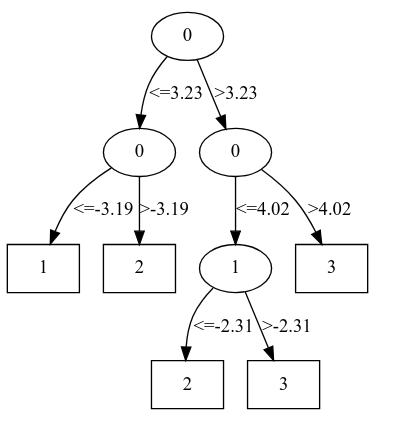
\includegraphics[width=.4\textwidth]{rsdm-tree-artificial.png}
	    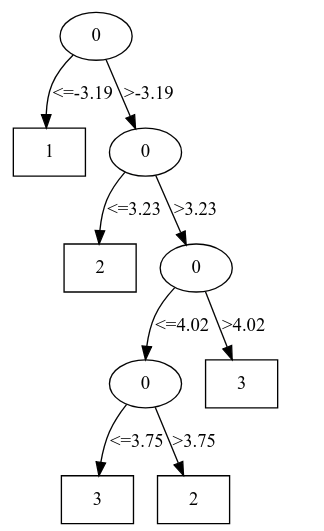
\includegraphics[width=.4\textwidth]{sdm-tree-artificial.png}
    \end{figure}
\end{frame}

\begin{frame}{RDMT(H) sur des datasets artificiels}

\end{frame}

\begin{frame}{RDMT(H) sur de vrais datasets}

\end{frame}

\begin{frame}[allowframebreaks]
  \printbibliography
\end{frame}

\end{document}
